\chapter{Конструкторский раздел}
\def \globalscale {1.0}

В данном разделе представлены схемы алгоритмов.

\section{Схемы алгоритмов модели освещения}

Схемы алгоритмов модели освещения представлены ниже.

\begin{enumerate}[label=\arabic*), labelsep=0.5em]
    \item Схема алгоритма Ламбертового освещения для точечного источника света (рисунок~\ref{chart:lambert_point}).
    \item Схема алгоритма Ламбертового освещения для прожекторного источника света (рисунок~\ref{chart:lambert_spot}).
\end{enumerate}

\begin{figure}
\centering
\begin{tikzpicture}[y=1cm, x=1cm, yscale=\globalscale,xscale=\globalscale, every node/.append style={scale=\globalscale}, inner sep=0pt, outer sep=0pt]
  \path[draw=black,miter limit=10.0,dash pattern=on 0.0794cm off 0.0794cm] (3.175, 15.1077) -- (3.7042, 15.1077);



  \path[draw=black,miter limit=10.0] (1.5875, 14.314) -- (1.5875, 13.7848);



  \path[draw=black,fill=white,rounded corners=0.8cm] (0.0, 15.9015) rectangle (3.175, 14.314);



  \begin{scope}[shift={(-0.0132, 0.0132)}]
    \node[text=black,anchor=south,fit={(0,0) (3.175, 1.5875)}] (text1662) at (1.5875, 15.0019){Начало};



  \end{scope}
  \path (3.7042, 16.4306) rectangle (4.736, 13.7848);



  \path[draw=black,miter limit=10.0] (4.736, 16.4306) -- (3.7042, 16.4306) -- (3.7042, 13.7848) -- (4.736, 13.7848);



  \begin{scope}[shift={(-0.0132, 0.0132)}]
    \node[text=black,anchor=south,fit={(0,0) (3.175, 1.5875)} ] (text6565) at (5.5, 15.0019){Алгоритм Ламбертового освещения для точечных источников света};



  \end{scope}
  \path[draw=black,miter limit=10.0] (1.5875, 12.4619) -- (1.5875, 11.9327);



  \path[draw=black,fill=white,miter limit=10.0] (0.5292, 13.7848) -- (2.6458, 13.7848) -- (3.175, 13.3615) -- (3.175, 12.4619) -- (0.0, 12.4619) -- (0.0, 13.3615) -- cycle;



  \begin{scope}[shift={(-0.0132, 0.0132)}]
    \node[text=black,anchor=south,fit={(0,0) (3.175, 1.5875)}] (text7727) at (1.5875, 13.0175){Обработка N пикселей};



  \end{scope}
  \path[draw=black,miter limit=10.0] (1.5875, 2.1677) -- (1.5875, 1.6386);



  \path[draw=black,fill=white,miter limit=10.0,cm={ -1.0,-0.0,0.0,-1.0,(3.175, 5.6584)}] (0.5292, 3.4906) -- (2.6458, 3.4906) -- (3.175, 3.0673) -- (3.175, 2.1677) -- (0.0, 2.1677) -- (0.0, 3.0673) -- cycle;



  \begin{scope}[shift={(-0.0132, 0.0132)}]
    \node[text=black,anchor=south,fit={(0,0) (3.175, 1.5875)}] (text9988) at (1.5875, 2.7252){Пока остались необработанные пиксели};



  \end{scope}
  \path[draw=black,miter limit=10.0] (1.5875, 10.3452) -- (1.5875, 9.816);



  \path[draw=black,miter limit=10.0,dash pattern=on 0.0794cm off 0.0794cm] (3.175, 11.139) -- (3.7042, 11.139);



  \path[draw=black,fill=white] (0.0, 11.9327) rectangle (3.175, 10.3452);



  \begin{scope}[shift={(-0.0132, 0.0132)}]
    \node[text=black,anchor=south,fit={(0,0) (3.175, 1.5875)}] (text7296) at (1.5875, 11.0331){$\vec{L}=norm(\vec{P_l}-\vec{P_f})$};



  \end{scope}
  \path[draw=black,miter limit=10.0,dash pattern=on 0.0794cm off 0.0794cm] (3.175, 9.0091) -- (3.7042, 9.0091);



  \path[draw=black,miter limit=10.0] (1.5875, 8.2153) -- (1.5875, 7.6994);



  \path[draw=black,fill=white] (0.0, 9.8028) rectangle (3.175, 8.2153);



  \begin{scope}[shift={(-0.0132, 0.0132)}]
    \node[text=black,anchor=south,fit={(0,0) (3.175, 1.5875)}] (text6853) at (1.5875, 8.9165){$I_{\text{diff}}=\max\begin{cases}\vec{L} \cdot \vec{N} \\ 0\end{cases}$};



  \end{scope}
  \path[draw=black,fill=white,rounded corners=0.8cm] (0.0, 1.6386) rectangle (3.175, 0.0511);



  \begin{scope}[shift={(-0.0132, 0.0132)}]
    \node[text=black,anchor=south,fit={(0,0) (3.175, 1.5875)}] (text6673) at (1.5875, 0.7408){Конец};



  \end{scope}
  \path (3.7042, 11.9081) rectangle (4.736, 10.3698);



  \path[draw=black,miter limit=10.0] (4.736, 11.9081) -- (3.7042, 11.9081) -- (3.7042, 10.3698) -- (4.736, 10.3698);



  \begin{scope}[shift={(-0.0132, 0.0132)}]
    \node[text=black,anchor=south,fit={(0,0) (3.175, 1.5875)} ] (text6100) at (5.5, 11.0331){Вычисление направления от пикселя к источнику света};



  \end{scope}
  \path (3.7042, 9.7782) rectangle (4.736, 8.2399);



  \path[draw=black,miter limit=10.0] (4.736, 9.7782) -- (3.7042, 9.7782) -- (3.7042, 8.2399) -- (4.736, 8.2399);



  \begin{scope}[shift={(-0.0132, 0.0132)}]
    \node[text=black,anchor=south,fit={(0,0) (3.175, 1.5875)} ] (text9922) at (5.5, 8.9165){Вычисление косинуса угла между нормалью и вектором $\vec{L}$};



  \end{scope}
  \path[draw=black,miter limit=10.0,dash pattern=on 0.0794cm off 0.0794cm] (3.175, 6.8908) -- (3.7042, 6.8858);



  \path[draw=black,miter limit=10.0] (1.5875, 6.1119) -- (1.5875, 5.6073);



  \path[draw=black,fill=white] (0.0, 7.6994) rectangle (3.175, 6.1119);



  \begin{scope}[shift={(-0.0132, 0.0132)}]
    \node[text=black,anchor=south,fit={(0,0) (3.175, 1.5875)}] (text8692) at (1.5875, 6.7998){$A=\max\begin{cases}1 - \frac{I_{\text{diff}}}{R} \\0\end{cases}$};



  \end{scope}
  \path (3.7042, 7.6502) rectangle (4.736, 6.1119);



  \path[draw=black,miter limit=10.0] (4.736, 7.6502) -- (3.7042, 7.6502) -- (3.7042, 6.1119) -- (4.736, 6.1119);



  \begin{scope}[shift={(-0.0132, 0.0132)}]
    \node[text=black,anchor=south,fit={(0,0) (3.175, 1.5875)} ] (text9266) at (5, 6.7733){Уменьшение интенсивности с расстоянием};



  \end{scope}
  \path[draw=black,miter limit=10.0] (1.5875, 4.0198) -- (1.5875, 3.4906);



  \path[draw=black,miter limit=10.0,dash pattern=on 0.0794cm off 0.0794cm] (3.175, 4.7987) -- (3.7042, 4.7937);



  \path[draw=black,fill=white] (0.0, 5.6073) rectangle (3.175, 4.0198);



  \begin{scope}[shift={(-0.0132, 0.0132)}]
    \node[text=black,anchor=south,fit={(0,0) (3.175, 1.5875)}] (text8086) at (1.5875, 4.7096){$\text{LightColor} = \text{Color} \cdot \text{Intensity} \cdot A \cdot I_{\text{diff}}$};



  \end{scope}
  \path (3.7042, 5.5581) rectangle (4.736, 4.0198);



  \path[draw=black,miter limit=10.0] (4.736, 5.5581) -- (3.7042, 5.5581) -- (3.7042, 4.0198) -- (4.736, 4.0198);



  \begin{scope}[shift={(-0.0132, 0.0132)}]
    \node[text=black,anchor=south,fit={(0,0) (3.175, 1.5875)},scale=0.8] (text1543) at (5.5, 4.6831){Результирующий цвет, где Intensity -- интенсивность источника света, Color -- цвет света};



  \end{scope}

\end{tikzpicture}

\caption{Схема алгоритма Ламбертового освещения для точечного источника света}
\label{chart:lambert_point}

\end{figure}

\FloatBarrier
\begin{figure}
\centering
\begin{tikzpicture}[y=1cm, x=1cm, yscale=\globalscale,xscale=\globalscale, every node/.append style={scale=\globalscale}, inner sep=0pt, outer sep=0pt]
  \path[draw=black,miter limit=10.0,dash pattern=on 0.0794cm off 0.0794cm] (3.175, 19.4469) -- (3.7042, 19.4469);



  \path[draw=black,miter limit=10.0] (1.5875, 18.6531) -- (1.5875, 18.124);



  \path[draw=black,fill=white,rounded corners=0.4445cm] (0.0, 20.2406) rectangle (3.175, 18.6531);



  \begin{scope}[shift={(-0.0132, 0.0132)}]
    \node[text=black,anchor=south,fit={(0,0) (3.175, 1.5875)}] (text7994) at (1.5875, 19.341){Начало};



  \end{scope}
  \path (3.7042, 20.7698) rectangle (4.736, 18.124);



  \path[draw=black,miter limit=10.0] (4.736, 20.7698) -- (3.7042, 20.7698) -- (3.7042, 18.124) -- (4.736, 18.124);



  \begin{scope}[shift={(-0.0132, 0.0132)}]
    \node[text=black,anchor=south,fit={(0,0) (3.175, 1.5875)} ] (text3136) at (5.5, 19.341){Алгоритм Ламбертового освещения для прожекторных источников света};



  \end{scope}
  \path[draw=black,miter limit=10.0] (1.5875, 16.801) -- (1.5875, 16.2719);



  \path[draw=black,fill=white,miter limit=10.0] (0.5292, 18.124) -- (2.6458, 18.124) -- (3.175, 17.7006) -- (3.175, 16.801) -- (0.0, 16.801) -- (0.0, 17.7006) -- cycle;



  \begin{scope}[shift={(-0.0132, 0.0132)}]
    \node[text=black,anchor=south,fit={(0,0) (3.175, 1.5875)}] (text5489) at (1.5875, 17.3567){Обработка N пикселей};



  \end{scope}
  \path[draw=black,miter limit=10.0] (1.5875, 2.1431) -- (1.5875, 1.614);



  \path[draw=black,fill=white,miter limit=10.0,cm={ -1.0,-0.0,0.0,-1.0,(3.175, 5.6092)}] (0.5292, 3.466) -- (2.6458, 3.466) -- (3.175, 3.0427) -- (3.175, 2.1431) -- (0.0, 2.1431) -- (0.0, 3.0427) -- cycle;



  \begin{scope}[shift={(-0.0132, 0.0132)}]
    \node[text=black,anchor=south,fit={(0,0) (3.175, 1.5875)}] (text8859) at (1.5875, 2.6988){Пока остались необработанные пиксели};



  \end{scope}
  \path[draw=black,miter limit=10.0] (1.5875, 14.6844) -- (1.5875, 14.1552);



  \path[draw=black,miter limit=10.0,dash pattern=on 0.0794cm off 0.0794cm] (3.175, 15.4781) -- (3.7042, 15.4781);



  \path[draw=black,fill=white] (0.0, 16.2719) rectangle (3.175, 14.6844);



  \begin{scope}[shift={(-0.0132, 0.0132)}]
    \node[text=black,anchor=south,fit={(0,0) (3.175, 1.5875)}] (text5326) at (1.5875, 15.3723){$\vec{L}=norm(\vec{P_l}-\vec{P_f})$};



  \end{scope}
  \path[draw=black,miter limit=10.0,dash pattern=on 0.0794cm off 0.0794cm] (3.175, 13.3482) -- (3.7042, 13.3482);



  \path[draw=black,miter limit=10.0] (1.5875, 12.5545) -- (1.5875, 12.0385);



  \path[draw=black,fill=white] (0.0, 14.142) rectangle (3.175, 12.5545);



  \begin{scope}[shift={(-0.0132, 0.0132)}]
    \node[text=black,anchor=south,fit={(0,0) (3.175, 1.5875)}] (text4645) at (1.5875, 13.2556){$I_{\text{diff}}=\max\begin{cases}\vec{L} \cdot \vec{N} \\ 0\end{cases}$};



  \end{scope}
  \path[draw=black,fill=white,rounded corners=0.4445cm] (0.0, 1.614) rectangle (3.175, 0.0265);



  \begin{scope}[shift={(-0.0132, 0.0132)}]
    \node[text=black,anchor=south,fit={(0,0) (3.175, 1.5875)}] (text1473) at (1.5875, 0.7144){Конец};



  \end{scope}
  \path (3.7042, 16.2473) rectangle (4.736, 14.709);



  \path[draw=black,miter limit=10.0] (4.736, 16.2473) -- (3.7042, 16.2473) -- (3.7042, 14.709) -- (4.736, 14.709);



  \begin{scope}[shift={(-0.0132, 0.0132)}]
    \node[text=black,anchor=south,fit={(0,0) (3.175, 1.5875)} ] (text1261) at (5.5, 15.3723){Вычисление
    направления от
    пикселя к источнику
    света};



  \end{scope}
  \path (3.7042, 14.1174) rectangle (4.736, 12.5791);



  \path[draw=black,miter limit=10.0] (4.736, 14.1174) -- (3.7042, 14.1174) -- (3.7042, 12.5791) -- (4.736, 12.5791);



  \begin{scope}[shift={(-0.0132, 0.0132)}]
    \node[text=black,anchor=south,fit={(0,0) (3.175, 1.5875)} ] (text5090) at (5.5, 13.2556){Вычисление косинуса угла между нормалью и вектором $\vec{L}$};



  \end{scope}
  \path[draw=black,miter limit=10.0,dash pattern=on 0.0794cm off 0.0794cm] (3.175, 11.23) -- (3.7042, 11.2249);



  \path[draw=black,miter limit=10.0] (1.5875, 10.451) -- (1.5875, 9.816);



  \path[draw=black,fill=white] (0.0, 12.0385) rectangle (3.175, 10.451);



  \begin{scope}[shift={(-0.0132, 0.0132)}]
    \node[text=black,anchor=south,fit={(0,0) (3.175, 1.5875)}] (text656) at (1.5875, 11.139){$A=\max\begin{cases}1 - \frac{I_{\text{diff}}}{R} \\0\end{cases}$};



  \end{scope}
  \path (3.7042, 11.9893) rectangle (4.736, 10.451);



  \path[draw=black,miter limit=10.0] (4.736, 11.9893) -- (3.7042, 11.9893) -- (3.7042, 10.451) -- (4.736, 10.451);



  \begin{scope}[shift={(-0.0132, 0.0132)}]
    \node[text=black,anchor=south,fit={(0,0) (3.175, 1.5875)} ] (text2294) at (5, 11.1125){Уменьшение интенсивности с расстоянием};



  \end{scope}
  \path[draw=black,miter limit=10.0] (1.5875, 3.9952) -- (1.5875, 3.466);



  \path[draw=black,miter limit=10.0,dash pattern=on 0.0794cm off 0.0794cm] (3.175, 4.7741) -- (3.7042, 4.7691);



  \path[draw=black,fill=white] (0.0, 5.5827) rectangle (3.175, 3.9952);



  \begin{scope}[shift={(-0.0132, 0.0132)}]
    \node[text=black,anchor=south,fit={(0,0) (3.175, 1.5875)}] (text2834) at (1.5875, 4.6831){$\text{LightColor} = \text{Color} \cdot \text{Intensity} \cdot \text{spotIntensity} \cdot A \cdot I_{\text{diff}}$};



  \end{scope}
  \path (3.7042, 5.5335) rectangle (4.736, 3.9952);



  \path[draw=black,miter limit=10.0] (4.736, 5.5335) -- (3.7042, 5.5335) -- (3.7042, 3.9952) -- (4.736, 3.9952);



  \begin{scope}[shift={(-0.0132, 0.0132)}]
    \node[text=black,anchor=south,fit={(0,0) (3.175, 1.5875)},scale=0.8] (text3823) at (5.5, 4.6567){Результирующий цвет, где Intensity -- интенсивность источника света, Color -- цвет света};



  \end{scope}
  \path[draw=black,miter limit=10.0] (1.5875, 8.2285) -- (1.5875, 7.6994);



  \path[draw=black,miter limit=10.0,dash pattern=on 0.0794cm off 0.0794cm] (3.175, 9.0223) -- (3.7042, 9.0223);



  \path[draw=black,fill=white] (0.0, 9.816) rectangle (3.175, 8.2285);



  \begin{scope}[shift={(-0.0132, 0.0132)}]
    \node[text=black,anchor=south,fit={(0,0) (3.175, 1.5875)}] (text8314) at (1.5875, 8.9165){$\text{spotEffect} = \vec{D} \cdot (-\vec{L})$};



  \end{scope}
  \path[draw=black,miter limit=10.0] (1.5875, 6.1119) -- (1.5875, 5.5827);



  \path[draw=black,miter limit=10.0,dash pattern=on 0.0794cm off 0.0794cm] (3.175, 6.9056) -- (3.7042, 6.9056);



  \path[draw=black,fill=white] (0.0, 7.6994) rectangle (3.175, 6.1119);



  \begin{scope}[shift={(-0.0132, 0.0132)}]
    \node[text=black,anchor=south,fit={(0,0) (3.175, 1.5875)},scale=0.55] (text8183) at (1.5875, 6.7998)
    {
      $
      \text{spotIntensity} = \min
      \begin{cases}
          \max
          \begin{cases}
              \frac{\text{spotEffect} - \cos(\theta_{\text{outer}})}{\cos(\theta_{\text{inner}}) - \cos(\theta_{\text{outer}})} \\
              0
          \end{cases} \\
          1
      \end{cases}
      $
    };



  \end{scope}
  \path (3.7042, 9.7914) rectangle (4.6567, 8.2531);



  \path[draw=black,miter limit=10.0] (4.6567, 9.7914) -- (3.7042, 9.7914) -- (3.7042, 8.2531) -- (4.6567, 8.2531);



  \begin{scope}[shift={(-0.0132, 0.0132)}]
    \node[text=black,anchor=south,fit={(0,0) (3.175, 1.5875)} ] (text6054) at (5.5, 8.9165){Формирование направления интенсивности света прожектора};



  \end{scope}
  \path (3.7042, 7.6748) rectangle (4.6567, 6.1365);



  \path[draw=black,miter limit=10.0] (4.6567, 7.6748) -- (3.7042, 7.6748) -- (3.7042, 6.1365) -- (4.6567, 6.1365);



  \begin{scope}[shift={(-0.0132, 0.0132)}]
    \node[text=black,anchor=south,fit={(0,0) (3.175, 1.5875)} ] (text8697) at (5.5, 6.7998){Смягчение рассеивания обода прожекторного луча};



  \end{scope}

\end{tikzpicture}

\caption{Схема алгоритма Ламбертового освещения для прожекторного источника света}
\label{chart:lambert_spot}

\end{figure}

\FloatBarrier

\section{Схемы алгоритмов теневых карт}

Схемы алгоритмов теневых карт представлены ниже.

\begin{enumerate}[label=\arabic*), labelsep=0.5em]
    \item Схема алгоритма теневых карт (\hbox{рисунок~\ref{chart:shadow_map}}).
    \item Схема алгоритма теневых карт с фильтрацией (PCF) (\hbox{рисунок~\ref{chart:shadow_map_pcf}}).
    \item Схема алгоритма теневых карт с фильтрацией шумом (NOISE) (\hbox{рисунок~\ref{chart:shadow_map_noise}}).
    \item Схема алгоритма мягких теневых карт с фильтрацией (PCSS) (\hbox{рисунок~\ref{chart:shadow_map_pcss}}).
    \item Схема алгоритма мягких теневых карт с фильтрацией шумом \hbox{(PCSS-NOISE)} (\hbox{рисунок~\ref{chart:shadow_map_pcss_noise}}).
\end{enumerate}

\begin{figure}[h]
    \centering
    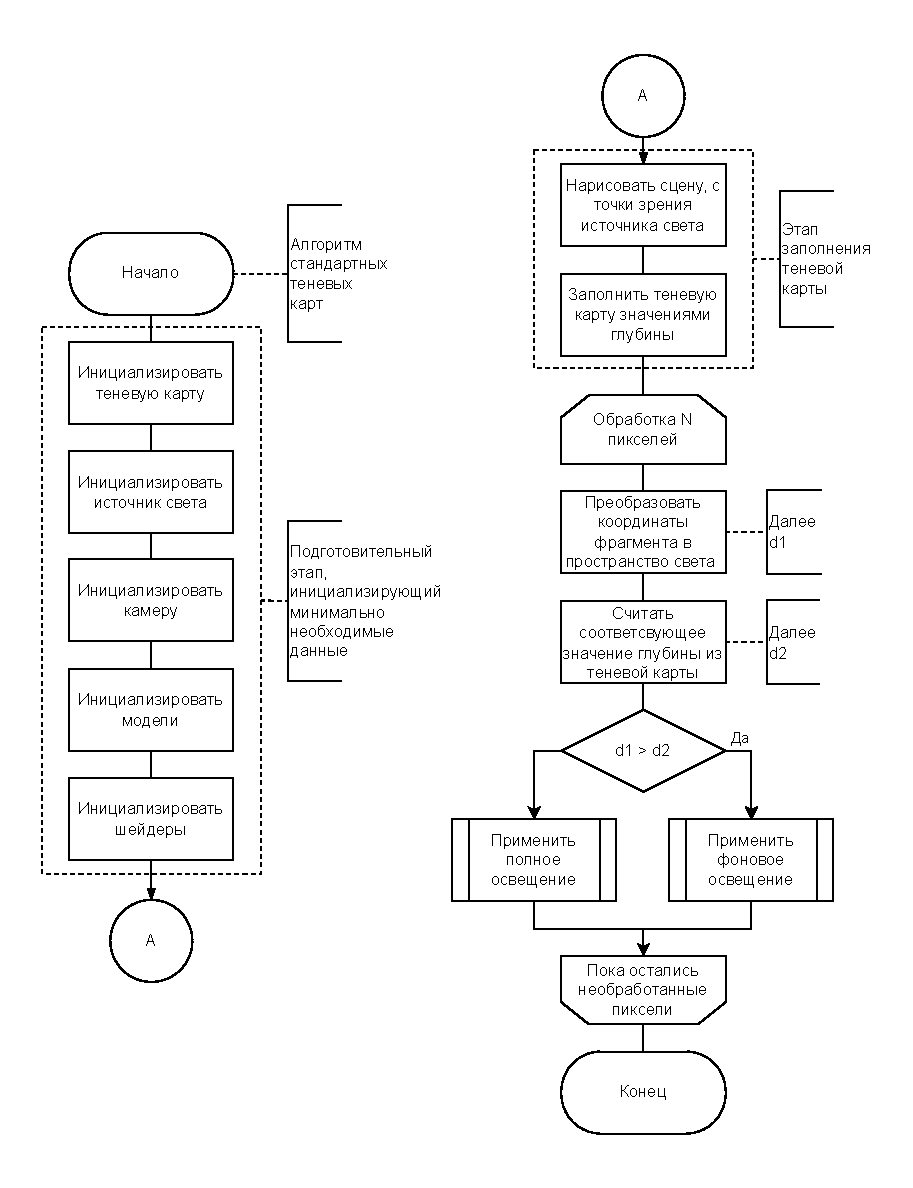
\includegraphics[width=\textwidth]{charts/shadow_map.pdf}
    \caption{Схема алгоритма теневых карт}
    \label{chart:shadow_map}
\end{figure}
\FloatBarrier
\begin{figure}[h]
    \centering
    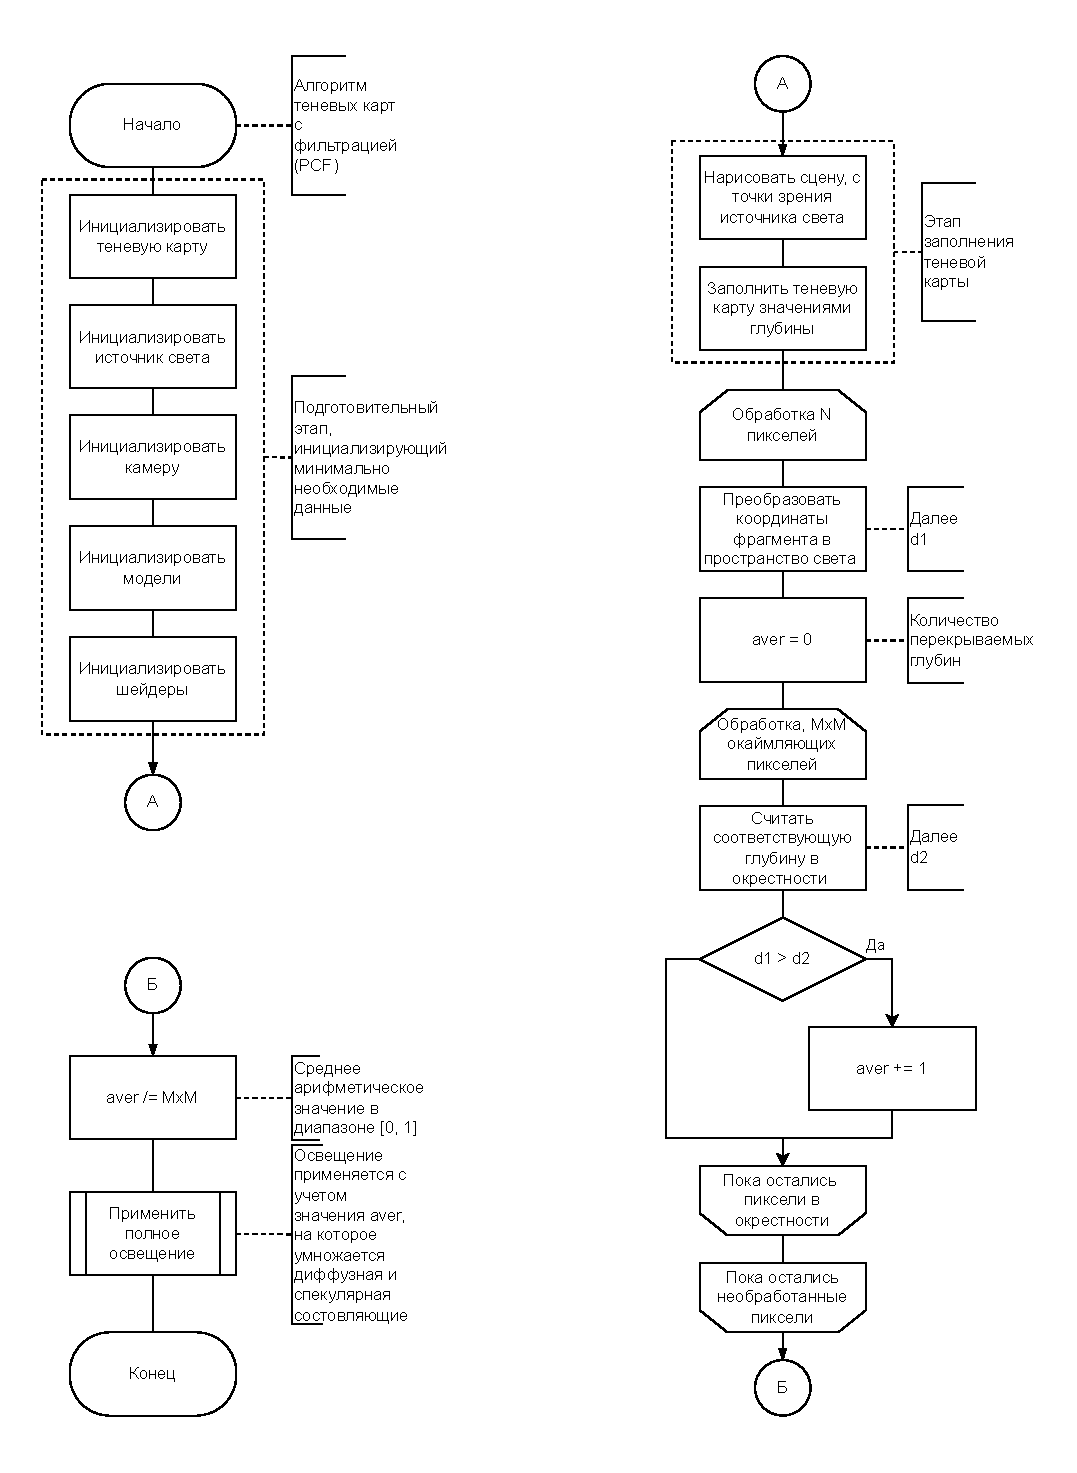
\includegraphics[width=\textwidth]{charts/shadow_map_pcf.pdf}
    \caption{Схема алгоритма теневых карт с линейной фильтрацией (PCF)}
    \label{chart:shadow_map_pcf}
\end{figure}
\FloatBarrier
\begin{figure}[h]
    \centering
    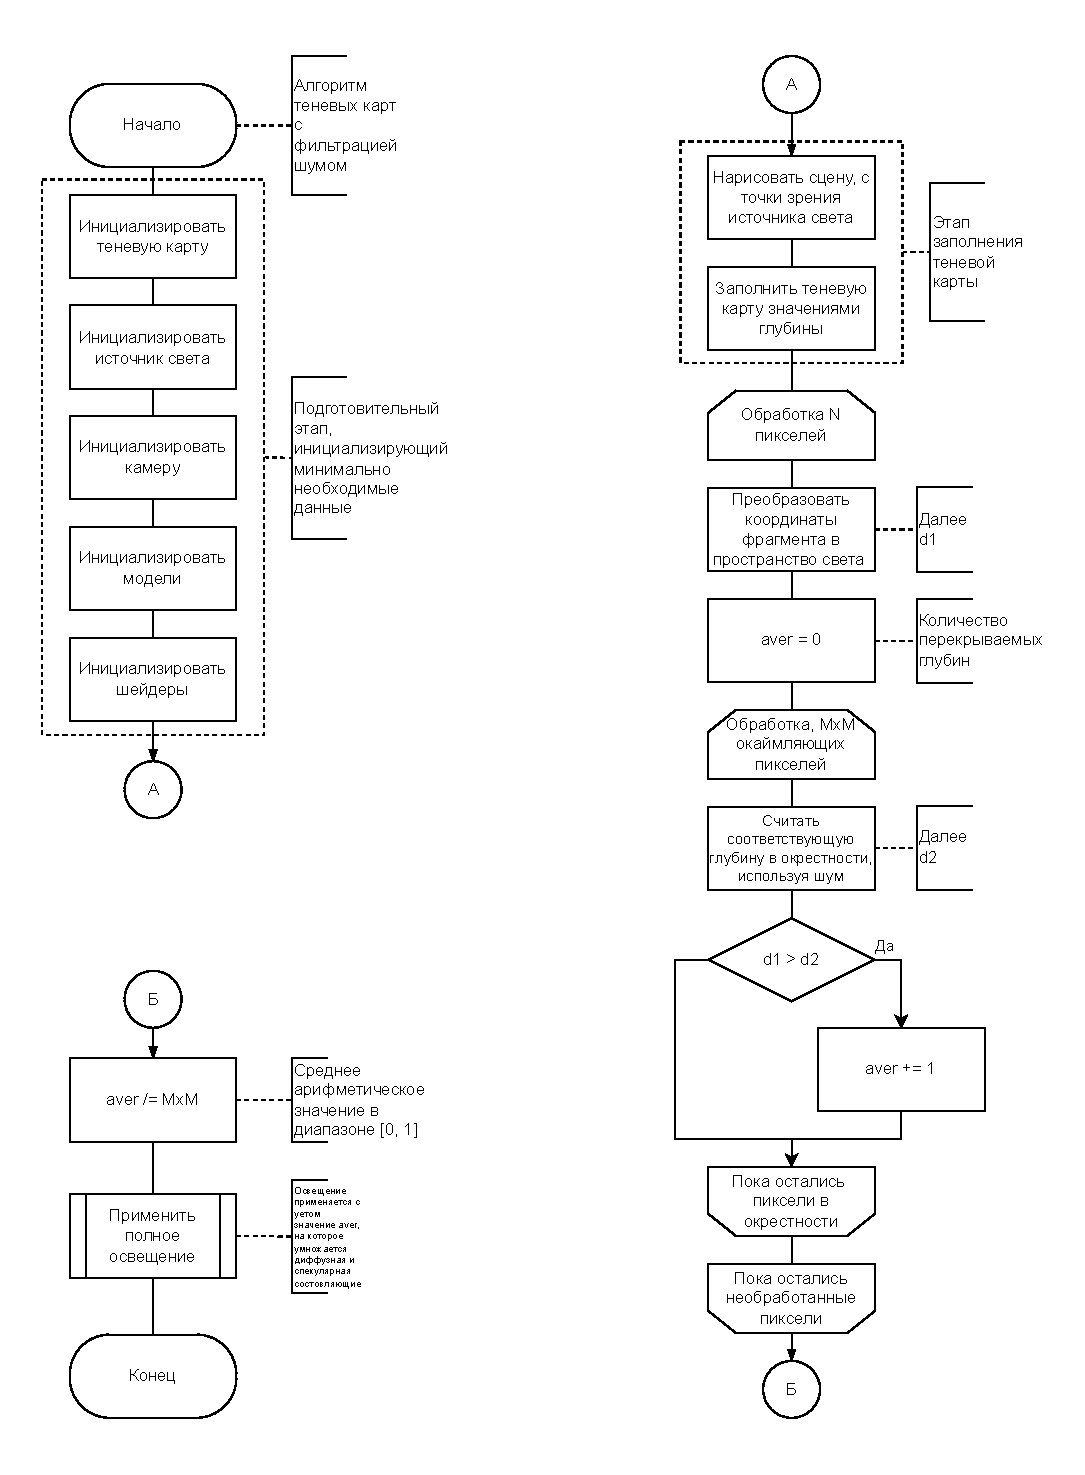
\includegraphics[width=\textwidth]{charts/shadow_map_noise.pdf}
    \caption{Схема алгоритма теневых карт с линейной фильтрацией шумом (NOISE)}
    \label{chart:shadow_map_noise}
\end{figure}
\FloatBarrier
\begin{figure}[h]
    \centering
    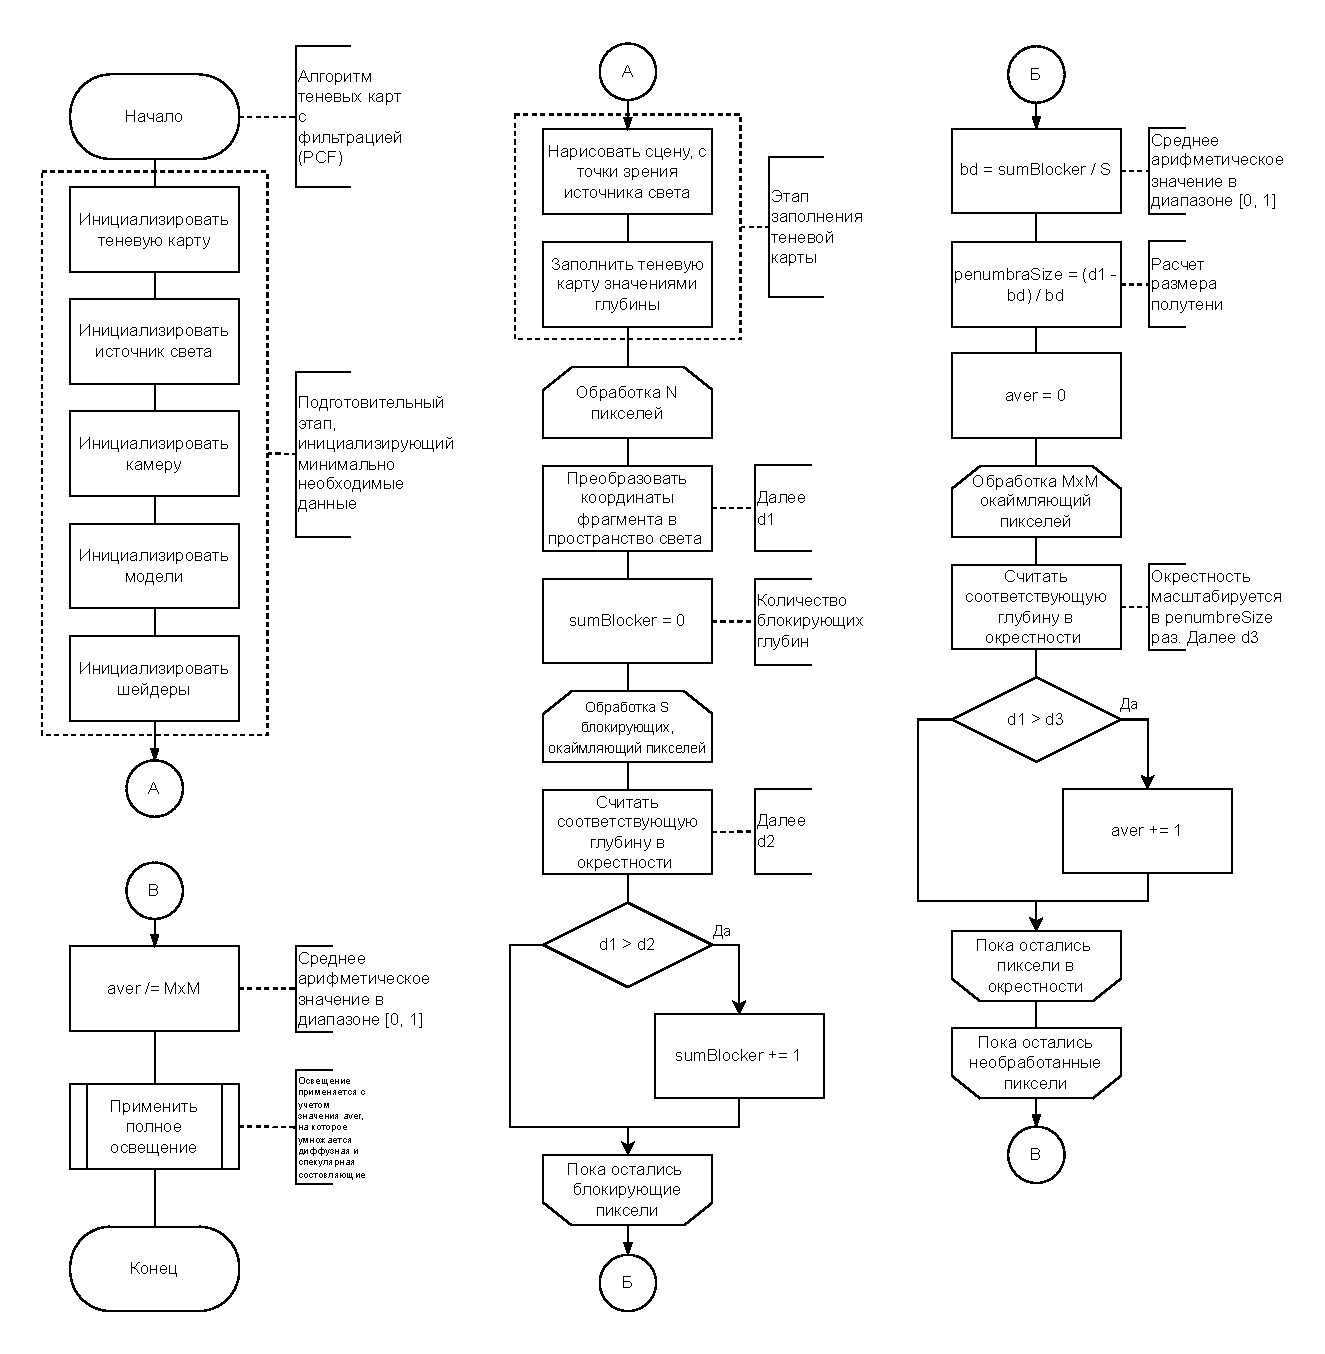
\includegraphics[width=\textwidth]{charts/shadow_map_pcss.pdf}
    \caption{Схема алгоритма мягких теневых карт с фильтрацией (PCSS)}
    \label{chart:shadow_map_pcss}
\end{figure}
\FloatBarrier
\begin{figure}[h]
    \centering
    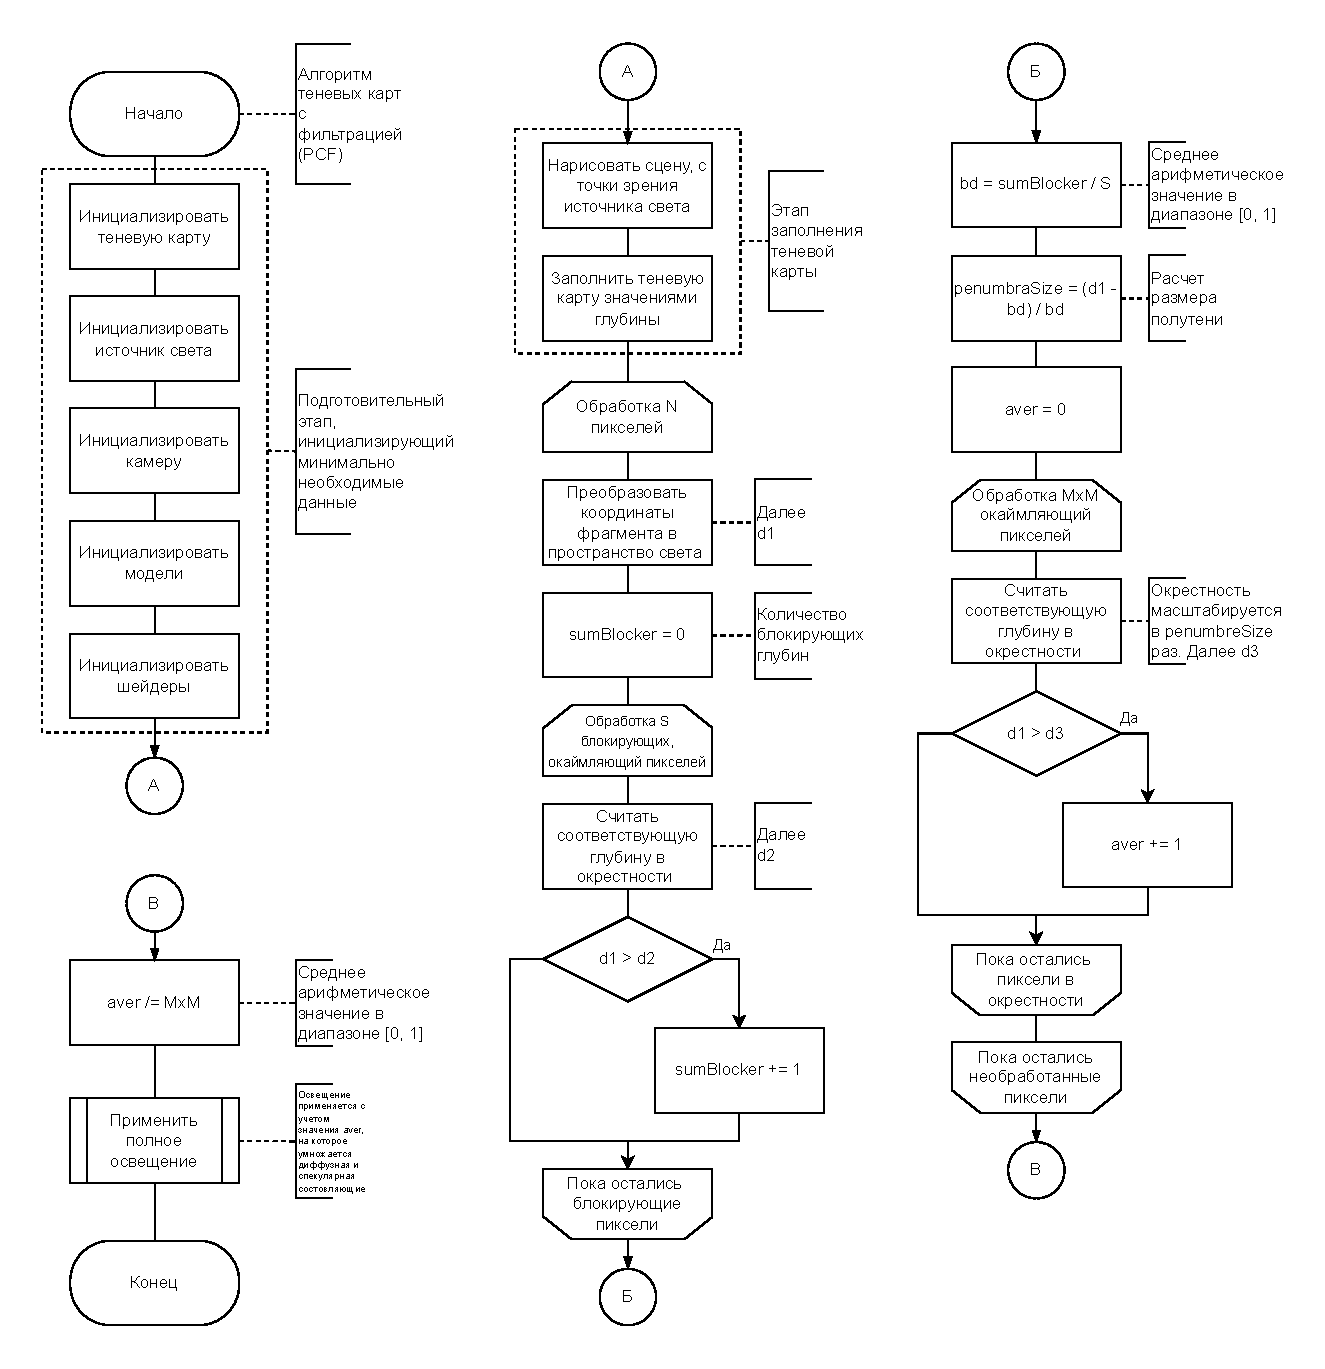
\includegraphics[width=\textwidth]{charts/shadow_map_pcss_noise.pdf}
    \caption{Схема алгоритма мягких теневых карт с фильтрацией шумом (PCSS-NOISE)}
    \label{chart:shadow_map_pcss_noise}
\end{figure}
\FloatBarrier

\section*{Вывод}

В данном разделе были представлены схемы алгоритмов модели освещения,
поддерживающей два источника света: точечный и прожекторный -- а также
схемы алгоритмов теневых карт.